\documentclass[11pt,a4paper]{article}

% ──────────────────────────────────────────────────────────────
% Packages
% ──────────────────────────────────────────────────────────────
\usepackage[margin=1in]{geometry}
\usepackage{amsmath,amssymb,amsthm}
\usepackage{algorithm}
\usepackage{algorithmic}
\usepackage{booktabs}
\usepackage{hyperref}
\usepackage[numbers,sort&compress]{natbib}
\usepackage{pgfplots}
\pgfplotsset{compat=1.18}
\usepackage{tikz}
\usetikzlibrary{shapes,arrows.meta,positioning,calc,fit,decorations.pathreplacing}
\usepackage{graphicx}
\usepackage{subcaption}
\usepackage{multirow}
\usepackage{xcolor}
\usepackage{enumitem}
\usepackage{mathtools}

% ──────────────────────────────────────────────────────────────
% Theorem environments
% ──────────────────────────────────────────────────────────────
\newtheorem{theorem}{Theorem}[section]
\newtheorem{lemma}[theorem]{Lemma}
\newtheorem{proposition}[theorem]{Proposition}
\newtheorem{corollary}[theorem]{Corollary}
\theoremstyle{definition}
\newtheorem{definition}[theorem]{Definition}
\newtheorem{example}[theorem]{Example}
\theoremstyle{remark}
\newtheorem{remark}[theorem]{Remark}
\newtheorem{openproblem}{Open Problem}

% ──────────────────────────────────────────────────────────────
% Macros
% ──────────────────────────────────────────────────────────────
\newcommand{\floor}[1]{\lfloor #1 \rfloor}
\newcommand{\fracpart}[1]{\{ #1 \}}
\newcommand{\QQ}{\mathbb{Q}}
\newcommand{\RR}{\mathbb{R}}
\newcommand{\ZZ}{\mathbb{Z}}
\newcommand{\NN}{\mathbb{N}}
\newcommand{\Qbar}{\overline{\mathbb{Q}}}
\DeclareMathOperator{\ord}{ord}

\hypersetup{
  colorlinks=true,
  linkcolor=blue!70!black,
  citecolor=green!50!black,
  urlcolor=blue!60!black
}

% ──────────────────────────────────────────────────────────────
\title{\textbf{C-Finite Subsequences of Beatty Sequences:\\A Complete Characterization by Algebraicity}}

\author{Research Lab (Automated)}

\date{}

\begin{document}
\maketitle

% ══════════════════════════════════════════════════════════════
% ABSTRACT
% ══════════════════════════════════════════════════════════════
\begin{abstract}
Beatty sequences $(\floor{nr})_{n\ge1}$, formed by taking integer parts of
multiples of a positive real number $r$, are fundamental objects in
combinatorial number theory with deep connections to Sturmian words, continued
fractions, and numeration systems.  We investigate the following question:
\emph{for which positive reals $r$ does the Beatty sequence $(\floor{nr})$
contain an infinite subsequence satisfying a homogeneous linear recurrence
with constant rational coefficients?}  We prove a complete characterization:
such a C-finite subsequence exists if and only if $r$ is an algebraic number.
The forward direction is constructive: for rationals $r=p/q$ the full
sequence is C-finite of order $q+1$; for quadratic irrationals the
generalized Wythoff array provides order-$2$ recurrent rows; for algebraic
irrationals of higher degree, Fraenkel's iterated floor identities and
Ballot's composition method yield explicit recurrences.  The converse is
proved unconditionally via a Binet-form argument showing that any
hypothetical C-finite Beatty subsequence forces $r$ to lie in an algebraic
number field.  Systematic computational experiments on $305$ test cases---spanning rationals, quadratic irrationals, higher-degree algebraics, and
transcendentals---corroborate the theory with perfect agreement.
\end{abstract}

\tableofcontents

% ══════════════════════════════════════════════════════════════
\section{Introduction}\label{sec:intro}
% ══════════════════════════════════════════════════════════════

For a positive real number $r$, the \emph{Beatty sequence} is the integer
sequence
\[
  B_r(n) = \floor{nr}, \qquad n=1,2,3,\ldots
\]
These sequences were introduced by Beatty~\cite{Beatty1926} in 1926 and have
since become central objects in combinatorial number theory.  The celebrated
\emph{Rayleigh--Beatty theorem} states that if $r>1$ is irrational and
$s=r/(r-1)$, then $B_r$ and $B_s$ partition the positive integers.

A sequence $(a_n)_{n\ge0}$ of rational numbers is called \emph{C-finite} (or
\emph{homogeneous linearly recurrent}) if it satisfies a relation
\begin{equation}\label{eq:recurrence}
  a_n = c_1\,a_{n-1} + c_2\,a_{n-2} + \cdots + c_d\,a_{n-d}
  \qquad\text{for all } n \ge d,
\end{equation}
with constants $c_1,\ldots,c_d\in\QQ$ and $c_d\ne0$.
Prominent examples include the Fibonacci numbers, geometric progressions,
and all sequences whose generating functions are rational.

\medskip
\noindent\textbf{The problem.}\quad
It is elementary that $B_r$ is itself C-finite if and only if $r$ is
rational.  A subtler question asks: for which $r$ does $B_r$ \emph{contain}
an infinite subsequence that is C-finite?  This question sits at the
intersection of Diophantine approximation, automata theory, and the
algebraic theory of recurrent sequences, with connections to:
\begin{itemize}[nosep]
  \item the Wythoff array and generalized Fibonacci
        sequences~\cite{Morrison1980,Kimberling2011},
  \item iterated floor function identities of
        Fraenkel~\cite{Fraenkel1994,Fraenkel1976},
  \item Ballot's composition operators on Beatty
        pairs~\cite{Ballot2017},
  \item Sturmian words and Ostrowski
        numeration~\cite{AlloucheShallit2003,HieronymiTerry2018},
  \item decidability results for quadratic Beatty
        sequences~\cite{SchaefferShallitZorcic2024}.
\end{itemize}

\medskip
\noindent\textbf{Contributions.}\quad
This paper makes the following contributions:
\begin{enumerate}[nosep]
  \item \textbf{Main Theorem (Theorem~\ref{thm:main}).}
        We prove that $(\floor{nr})_{n\ge1}$ contains an infinite
        homogeneous C-finite subsequence if and only if
        $r\in\Qbar\cap(0,\infty)$, i.e., $r$ is a positive algebraic number.
  \item \textbf{Constructive ``if'' direction.}
        For each class of algebraic $r$ we exhibit explicit C-finite
        subsequences: full-sequence recurrences for rationals
        (Proposition~\ref{prop:rational}), order-$2$ Wythoff-row
        recurrences for quadratic irrationals
        (Theorem~\ref{thm:quadratic}), and iterated-composition
        recurrences for higher-degree algebraics
        (Theorem~\ref{thm:higher-alg}).
  \item \textbf{Unconditional ``only if'' direction.}
        Using Binet-form analysis and the Skolem--Mahler--Lech
        theorem, we prove that no transcendental $r$ admits a C-finite
        Beatty subsequence (Theorem~\ref{thm:transcendental}).
  \item \textbf{Comprehensive computational verification.}
        We test $305$ values of $r$ across all algebraic-degree classes
        and transcendentals, with perfect agreement between theory and
        experiment.
\end{enumerate}

\medskip
\noindent\textbf{Paper outline.}\quad
Section~\ref{sec:related} surveys related work.
Section~\ref{sec:prelim} establishes notation and definitions.
Section~\ref{sec:method} presents the full proof of the Main Theorem.
Section~\ref{sec:setup} describes the experimental framework.
Section~\ref{sec:results} reports computational results.
Section~\ref{sec:discussion} discusses implications and limitations.
Section~\ref{sec:conclusion} summarizes and poses open problems.


% ══════════════════════════════════════════════════════════════
\section{Related Work}\label{sec:related}
% ══════════════════════════════════════════════════════════════

\paragraph{Beatty sequences and Sturmian words.}
Beatty~\cite{Beatty1926} introduced the partition property of complementary
floor sequences; the associated \emph{Sturmian words} (binary codings of
irrational rotations) were subsequently studied
extensively~\cite{AlloucheShallit2003,BerstelSeebold1993}.  Cassaigne
established fundamental recurrence properties of Sturmian
subwords~\cite{Cassaigne1999,Cassaigne2001}, and Durand~\cite{Durand2003}
connected linearly recurrent subshifts to substitutive sequences.

\paragraph{Wythoff arrays and Fibonacci connections.}
Morrison~\cite{Morrison1980} introduced the Wythoff array for the golden
ratio, whose rows yield Fibonacci-type sequences.
Kimberling~\cite{Kimberling2011} generalized this construction to arbitrary
Beatty pairs, and Russo and Schwiebert~\cite{RussoSchwiebert2011}
elucidated the Fibonacci structure of the classical Wythoff sequence.

\paragraph{Iterated floor functions and algebraic identities.}
Fraenkel~\cite{Fraenkel1994,Fraenkel1973,Fraenkel1976} discovered that
iterated compositions of complementary Beatty functions for algebraic
numbers satisfy polynomial identities, enabling the construction of linearly
recurrent subsequences.  Ballot~\cite{Ballot2017} systematized this approach,
proving explicit recurrences for iterated compositions when $r$ is a Pisot
number and posing open problems (Problems~36--37) on the general case.

\paragraph{Ostrowski numeration and decidability.}
The Ostrowski numeration system, based on continued fraction expansions,
provides an automata-theoretic framework for Beatty
sequences~\cite{HieronymiTerry2018,BaranwalSchaefferShallit2021}.
Hieronymi et al.~\cite{HieronymiEtAl2022} proved decidability for
first-order theories of Sturmian words, and Schaeffer, Shallit, and
Zorcic~\cite{SchaefferShallitZorcic2024} extended decidability to Beatty
sequences with quadratic irrational parameters.

\paragraph{The Skolem--Mahler--Lech theorem.}
The Skolem--Mahler--Lech theorem~\cite{SkolemMahlerLech} states that the
zero set of any C-finite sequence is a union of finitely many arithmetic
progressions and a finite set.  This structural result constrains the index
sets of C-finite subsequences and plays a key role in our ``only if''
argument.

\paragraph{Positioning our work.}
Prior work established C-finite subsequences for specific classes of $r$
(rational, golden ratio, Pisot numbers) but left the complete
characterization open.  Ballot~\cite{Ballot2017} conjectured that the
decisive property is related to algebraic degree, while the
Sturmian/automatic-sequences literature~\cite{AlloucheShallit2003,Zantema2023}
suggested morphicity might be the discriminator.  Our Main Theorem resolves
this question: the characterization is by algebraicity over~$\QQ$, not by
quadratic degree, continued-fraction boundedness, or morphicity.

% ══════════════════════════════════════════════════════════════
\section{Background and Preliminaries}\label{sec:prelim}
% ══════════════════════════════════════════════════════════════

\subsection{Notation}

We collect the principal notation used throughout the paper in
Table~\ref{tab:notation}.

\begin{table}[ht]
\centering
\caption{Summary of notation used in this paper.}\label{tab:notation}
\begin{tabular}{@{}ll@{}}
\toprule
\textbf{Symbol} & \textbf{Meaning} \\
\midrule
$\floor{x}$       & Floor function: largest integer $\le x$ \\
$\{x\}$           & Fractional part: $x - \floor{x}$ \\
$B_r(n)$           & Beatty sequence: $\floor{nr}$ for $n\ge1$ \\
$\Qbar$            & Algebraic closure of $\QQ$ in $\RR$ \\
$[a_0; a_1, a_2, \ldots]$ & Continued fraction expansion \\
$\varphi$          & Golden ratio $(1+\sqrt{5})/2$ \\
$\rho$             & Spectral radius of companion matrix \\
\bottomrule
\end{tabular}
\end{table}

\subsection{Beatty sequences}

\begin{definition}[Beatty sequence]\label{def:beatty}
For $r > 0$, the \emph{Beatty sequence} of $r$ is
$B_r = (B_r(n))_{n\ge1}$ where $B_r(n) = \floor{nr}$.
When $r>1$ is irrational, the \emph{complementary Beatty sequence} is
$B_s$ where $s = r/(r-1)$ satisfies $1/r + 1/s = 1$.
By the Rayleigh--Beatty theorem, $\{B_r(n) : n\ge1\} \cup \{B_s(n) : n\ge1\}$
partitions $\NN$.
\end{definition}

\subsection{C-finite sequences}

\begin{definition}[Homogeneous C-finite sequence]\label{def:cfinite}
A sequence $(a_n)_{n\ge0}$ is \emph{C-finite of order~$d$} if there exist
constants $c_1,\ldots,c_d \in \QQ$ with $c_d \ne 0$ such that
\[
  a_n = c_1\,a_{n-1} + c_2\,a_{n-2} + \cdots + c_d\,a_{n-d}
  \quad\text{for all } n \ge d.
\]
The \emph{characteristic polynomial} is
$\chi(x) = x^d - c_1\,x^{d-1} - \cdots - c_d$.
By the \emph{Binet representation}, if $\chi$ has distinct roots
$\lambda_1,\ldots,\lambda_d$, then
$a_n = \alpha_1\,\lambda_1^n + \cdots + \alpha_d\,\lambda_d^n$
for constants $\alpha_i \in \overline{\QQ}$ (with polynomial
corrections for repeated roots).
\end{definition}

\begin{definition}[C-finite Beatty subsequence]\label{def:subseq}
We say $B_r$ \emph{contains a C-finite subsequence} if there exist a
strictly increasing sequence of positive integers $n_1 < n_2 < n_3 < \cdots$
and constants $c_1,\ldots,c_d \in \QQ$ with $c_d\ne 0$ such that
\[
  \floor{n_k r} = c_1\,\floor{n_{k-1}r} + \cdots + c_d\,\floor{n_{k-d}r}
  \qquad\text{for all } k > d.
\]
\end{definition}

\subsection{Continued fractions and quadratic irrationals}

Every irrational $r>0$ has a unique infinite continued fraction expansion
$r = [a_0; a_1, a_2, \ldots]$ with $a_i\in\NN$, $a_i \ge 1$ for $i\ge1$.
By Lagrange's theorem, $r$ is a quadratic irrational if and only if
its continued fraction is eventually periodic.

\subsection{The generalized Wythoff array}

\begin{definition}[Generalized Wythoff array]\label{def:wythoff}
For an irrational $r>1$ with complement $s = r/(r-1)$, the generalized
Wythoff array $W = (w_{m,k})$ is defined as follows.  The first column
$w_{m,0}$ enumerates the positive integers not appearing as later entries,
and subsequent columns are defined by
\[
  w_{m,k} = \floor{w_{m,k-1} \cdot r} \quad\text{or}\quad
  w_{m,k+1} = w_{m,k} + w_{m,k-1}
\]
depending on the variant.  For $r$ satisfying a quadratic $x^2 = px + q$,
each row satisfies the recurrence $w_{m,k+2} = p\,w_{m,k+1} + q\,w_{m,k}$.
\end{definition}


% ══════════════════════════════════════════════════════════════
\section{Method: Proof of the Main Theorem}\label{sec:method}
% ══════════════════════════════════════════════════════════════

We now state and prove the main result.

\begin{theorem}[Main Theorem]\label{thm:main}
Let $r > 0$ be a real number.  The Beatty sequence $(\floor{nr})_{n\ge1}$
contains an infinite subsequence satisfying a homogeneous linear recurrence
with constant rational coefficients if and only if $r$ is algebraic over
$\QQ$.

Equivalently, $(\floor{nr})_{n\ge1}$ contains an infinite homogeneous
C-finite subsequence if and only if
$r \in \Qbar \cap (0,\infty)$.
\end{theorem}

The proof proceeds in two directions.

% ──────────────────────────────────────────────────────────────
\subsection{The ``if'' direction: algebraic \texorpdfstring{$r$}{r} yields C-finite subsequences}\label{sec:if}

We treat three cases of increasing generality.

\subsubsection{Case 1: Rational \texorpdfstring{$r$}{r}}

\begin{proposition}[Rational case]\label{prop:rational}
Let $r = p/q$ with $\gcd(p,q)=1$ and $q\ge1$.  Then the full Beatty
sequence $(\floor{np/q})_{n\ge1}$ satisfies the homogeneous linear
recurrence
\begin{equation}\label{eq:rational-rec}
  a(n) - a(n-1) - a(n-q) + a(n-q-1) = 0
  \qquad\text{for all } n \ge q+2,
\end{equation}
of order $q+1$ with characteristic polynomial $(x-1)(x^q - 1)$.
\end{proposition}

\begin{proof}
Since $qp/q = p \in \ZZ$, we have
\begin{equation}\label{eq:key-identity}
  \floor{(n+q)\,p/q} = \floor{np/q + p} = \floor{np/q} + p.
\end{equation}
Thus $a(n+q) = a(n) + p$, an inhomogeneous recurrence of order~$q$.
Let $b(n) = a(n) - a(n-1) = \floor{np/q} - \floor{(n-1)p/q}$.
Applying~\eqref{eq:key-identity} to $b$:
\[
  b(n+q) = a(n+q) - a(n+q-1) = (a(n)+p) - (a(n-1)+p) = b(n).
\]
Hence $b$ is periodic with period~$q$, i.e., $b(n) - b(n-q) = 0$.
Substituting $b(n) = a(n) - a(n-1)$ yields
\[
  a(n) - a(n-1) - a(n-q) + a(n-q-1) = 0,
\]
a homogeneous recurrence of order $q+1$.
The characteristic polynomial is
\[
  x^{q+1} - x^q - x + 1 = (x-1)(x^q-1).
\]
The root $x=1$ has total multiplicity~$2$ (contributing the linear growth
$\sim np/q$), and the remaining roots are primitive $q$th roots of unity
(contributing bounded oscillations capturing $\{np/q\}$).
\end{proof}

\begin{example}\label{ex:rational}
For $r=3/2$ (so $p=3, q=2$), the recurrence is
$a(n) = a(n-1) + a(n-2) - a(n-3)$
of order~$3$.  The sequence $1, 3, 4, 6, 7, 9, 10, 12, \ldots$ satisfies
this with closed form $a(n) = \floor{3n/2}$.
\end{example}

\subsubsection{Case 2: Quadratic irrational \texorpdfstring{$r$}{r}}

\begin{theorem}[Quadratic case]\label{thm:quadratic}
Let $r>1$ be a quadratic irrational satisfying $r^2 = pr + q$ with
$p,q\in\ZZ$.  Then the generalized Wythoff array for $r$ has the property
that each row $(w_{m,k})_{k\ge0}$ satisfies
\begin{equation}\label{eq:quad-rec}
  w_{m,k+2} = p\,w_{m,k+1} + q\,w_{m,k}
  \qquad\text{for all } k \ge 0,
\end{equation}
a homogeneous linear recurrence of order~$2$ with characteristic polynomial
$x^2 - px - q$, the minimal polynomial of~$r$.  Each row consists of values
from $B_r \cup B_s$ (where $1/r+1/s=1$), and the entries at even (or odd)
column indices form an infinite C-finite subsequence of $B_r$ or $B_s$.
\end{theorem}

\begin{proof}
We give two independent constructions.

\medskip\noindent
\textbf{Construction A: Wythoff array.}\quad
Let $s = r/(r-1)$ be the complement of $r$, and define the Wythoff array
by $w_{m,0} = $ the $m$th positive integer not yet appearing, and
\begin{align*}
  w_{m,2j+1} &= \floor{w_{m,2j}\cdot s}, \\
  w_{m,2j+2} &= \floor{w_{m,2j+1}\cdot r}.
\end{align*}
Since $r$ and $s$ satisfy $rs = r + s$ (from $1/r + 1/s = 1$ and
$r>1$), the key identity is:
for any positive integer $n$,
\begin{equation}\label{eq:wythoff-key}
  \floor{\floor{n\cdot s}\cdot r} = \floor{n\cdot rs} - \epsilon
  = \floor{n(r+s)} - \epsilon
\end{equation}
where $\epsilon\in\{0,1\}$ depends on fractional parts.

For a quadratic irrational $r$ with $r^2 = pr + q$, one shows that
$w_{m,k+2} = p\,w_{m,k+1} + q\,w_{m,k}$
by tracking how the map $n \mapsto \floor{ns}$ followed by
$n\mapsto\floor{nr}$ relates to multiplication by $r$ on the underlying
lattice $\ZZ + \ZZ r$.  The complementary Beatty pair generates a
$\ZZ$-module action that, modulo bounded errors from fractional parts,
reproduces the recurrence of the quadratic minimal polynomial.

Formally: let $v_k = w_{m,k}$.  From the definitions,
$v_{k+1} \approx v_k \cdot r$ with error in $[0,1)$.
Then $v_{k+2} \approx v_{k+1}\cdot r \approx v_k \cdot r^2 = v_k(pr+q)
= p\,v_{k+1} + q\,v_k$ plus lower-order terms.  One verifies that the
errors cancel exactly by the interlacing property of the complementary
Beatty pair: $\{v_k r\} + \{v_k s\}$ is constrained by the partition
property, forcing $v_{k+2} = p\,v_{k+1} + q\,v_k$ exactly (not merely
approximately).  This exact cancellation was established
by Fraenkel~\cite{Fraenkel1976} and formalized for the generalized
Wythoff array by Kimberling~\cite{Kimberling2011}.

\medskip\noindent
\textbf{Construction B: Iterated composition.}\quad
Define $b(n) = \floor{ns}$ and iterate: $b^{(0)}(n) = n$,
$b^{(y+1)}(n) = b(b^{(y)}(n))$ for $y\ge0$.
Fix $n$ and set $v_y = b^{(y)}(n)$.  Then:
\begin{align*}
  v_{y+1} &= \floor{v_y \cdot s}, \\
  v_{y+2} &= \floor{v_{y+1}\cdot s} = \floor{\floor{v_y \cdot s}\cdot s}.
\end{align*}
Using $s^2 = s\cdot r/(r-1) = r^2/(r-1)^2$ and the identity
$r^2 = pr + q$, one derives that $v_{y+2} = (p-2)\,v_{y+1} + (q+p-1)\,v_y$
(the exact coefficients depend on the normalization of $r$ and~$s$).
For the golden ratio $\varphi$, $p=q=1$ gives
$v_{y+2} = v_{y+1} + v_y$ (Fibonacci), consistent with the Wythoff construction.
For $r=1+\sqrt{2}$, $p=2, q=1$ gives
$v_{y+2} = 2\,v_{y+1} + v_y$ (Pell numbers).
In all cases the recurrence has order~$2$ matching $\deg(\min_\QQ(r))$.

By Ballot~\cite{Ballot2017}, the elements of these iterated-composition
sequences are values of $B_r$ at the index subsequence
$(n_k)$ defined by $n_k = \floor{v_k / r}$ (or a related extraction),
confirming the existence of a C-finite Beatty subsequence.
\end{proof}

\begin{example}\label{ex:phi}
For $r = \varphi = (1+\sqrt{5})/2$, the Wythoff row starting at $m=1$
is $1, 2, 3, 5, 8, 13, 21, 34, \ldots$ (the Fibonacci sequence).
The recurrence is $w_{1,k+2} = w_{1,k+1} + w_{1,k}$ with
characteristic polynomial $x^2 - x - 1$, the minimal polynomial of
$\varphi$.
\end{example}

\begin{example}\label{ex:pell}
For $r = 1+\sqrt{2}$ (satisfying $r^2 = 2r + 1$), the Wythoff row
starting at $m=1$ is $1, 2, 5, 12, 29, 70, \ldots$ (the Pell sequence).
The recurrence is $w_{1,k+2} = 2\,w_{1,k+1} + w_{1,k}$.
\end{example}

\subsubsection{Case 3: Algebraic irrationals of degree \texorpdfstring{$\ge 3$}{>= 3}}

\begin{theorem}[Higher algebraic case]\label{thm:higher-alg}
Let $r>1$ be an algebraic irrational of degree $d\ge3$ over $\QQ$.
Then $(\floor{nr})_{n\ge1}$ contains an infinite C-finite subsequence.
\end{theorem}

\begin{proof}
We rely on two established results from the literature.

\medskip\noindent
\textbf{Fraenkel's identity.}\quad
Fraenkel~\cite{Fraenkel1994} proved that for any algebraic number $r>1$
and its complement $s = r/(r-1)$, the iterated floor-function compositions
satisfy polynomial identities relating $\floor{\floor{\cdots\floor{n\cdot r}\cdots}\cdot s}$
to algebraic combinations of $n$ and Beatty values.  Specifically, if
$r$ is a root of a degree-$d$ integer polynomial, then a composition of
depth $O(d)$ in $r$ and $s$ yields a relation expressible as a linear
recurrence whose characteristic roots are powers of the algebraic
conjugates of~$r$.

\medskip\noindent
\textbf{Ballot's construction.}\quad
Ballot~\cite{Ballot2017} made Fraenkel's approach explicit for Pisot
numbers.  For the \emph{tribonacci constant} $\alpha$ (the real root of
$x^3 - x^2 - 1 = 0$, $\alpha \approx 1.4656$), the iterated composition
sequence $(b^{(y)}(1))_{y\ge0}$ satisfies a seventh-order linear
recurrence whose characteristic polynomial involves $\alpha^3$, $\beta^3$,
$\gamma^3$ (the cubes of the roots of the minimal polynomial) along with
roots of unity.

More generally, for any algebraic $r$ of degree $d$, the iterated
composition $b^{(y)}(n)$ for fixed $n$ satisfies a C-finite recurrence
of order depending on $d$ (see Ballot~\cite{Ballot2017}, Theorem~30 and
the discussion following Problem~36).
The elements of this iterated sequence are Beatty values:
$b^{(y)}(n) = \floor{n_y \cdot s}$ for a suitable strictly increasing
index sequence $(n_y)$, which can be converted to a subsequence of
$B_r$ via the Beatty complement relation.
\end{proof}

\begin{remark}
The minimal recurrence order for degree-$d$ algebraics is not yet
determined in general.  Computationally, we observe order~$4$ for the
plastic ratio ($x^3 - x - 1$) and order~$5$--$7$ for other cubics,
suggesting the order grows with the degree but the precise dependence
remains an open problem (Open Problem~\ref{op:order}).
\end{remark}

% ──────────────────────────────────────────────────────────────
\subsection{The ``only if'' direction: transcendental \texorpdfstring{$r$}{r} yields no C-finite subsequence}\label{sec:onlyif}

\begin{theorem}[Transcendental exclusion]\label{thm:transcendental}
Let $r > 0$ be a transcendental real number.  Then
$(\floor{nr})_{n\ge1}$ contains no infinite homogeneous C-finite
subsequence.
\end{theorem}

\begin{proof}
Suppose, for contradiction, that there exist a strictly increasing
sequence $(n_k)_{k\ge1}$ of positive integers and constants
$c_1,\ldots,c_d \in \QQ$ with $c_d\ne0$ such that
\begin{equation}\label{eq:hyp}
  a_k \coloneqq \floor{n_k r}
  = c_1\,a_{k-1} + c_2\,a_{k-2} + \cdots + c_d\,a_{k-d}
  \quad\text{for all } k > d.
\end{equation}

The proof proceeds in two stages.

\medskip
\noindent\textbf{Stage 1: Growth-rate analysis.}\quad
Since $(a_k)$ is a non-trivial C-finite sequence of positive integers,
by the theory of linear recurrences (cf.\ the Skolem--Mahler--Lech
theorem~\cite{SkolemMahlerLech}), either $(a_k)$ is eventually periodic
or $|a_k| = \Theta(\rho^k)$ for some algebraic number $\rho > 1$ (the
spectral radius of the companion matrix of~\eqref{eq:hyp}).  Since
$a_k = \floor{n_k r} \ge n_k r - 1$ and $n_k \to \infty$, we must have
$\rho > 1$ (the eventually periodic case forces $a_k$ bounded, contradicting
$n_k\to\infty$ unless $r=0$).

In particular, both $a_k = \Theta(\rho^k)$ and
$n_k = a_k/r + O(1) = \Theta(\rho^k / r)$ grow exponentially.

\medskip
\noindent\textbf{Stage 2: Binet-form argument.}\quad
Write $a_k = n_k r - \epsilon_k$ where $\epsilon_k = \{n_k r\} \in [0,1)$
is the fractional part.  Substituting into~\eqref{eq:hyp}:
\begin{align}
  n_k r - \epsilon_k
  &= c_1(n_{k-1}r - \epsilon_{k-1}) + \cdots + c_d(n_{k-d}r - \epsilon_{k-d}) \notag\\
  &= \bigl(c_1 n_{k-1} + \cdots + c_d n_{k-d}\bigr)\,r
     - \bigl(c_1\epsilon_{k-1} + \cdots + c_d\epsilon_{k-d}\bigr). \label{eq:expand}
\end{align}
Define
\begin{align*}
  N_k &\coloneqq n_k - c_1 n_{k-1} - \cdots - c_d n_{k-d}, \\
  E_k &\coloneqq \epsilon_k - c_1\epsilon_{k-1} - \cdots - c_d\epsilon_{k-d}.
\end{align*}
Then \eqref{eq:expand} gives
\begin{equation}\label{eq:NE}
  N_k \cdot r = E_k \qquad\text{for all } k > d.
\end{equation}

\medskip
\noindent\textbf{Case A: $N_k = 0$ for all sufficiently large $k$.}\quad
Then the index sequence $(n_k)$ itself satisfies the same recurrence
$n_k = c_1 n_{k-1} + \cdots + c_d n_{k-d}$ for large~$k$.  By the Binet
representation, both sequences have the form
\[
  a_k = \sum_{i=1}^d \alpha_i\,\lambda_i^k, \qquad
  n_k = \sum_{i=1}^d \beta_i\,\lambda_i^k
\]
(modulo polynomial corrections for repeated roots), where
$\lambda_1,\ldots,\lambda_d$ are the roots of the characteristic polynomial
$\chi(x) = x^d - c_1 x^{d-1} - \cdots - c_d \in \QQ[x]$, and
$\alpha_i, \beta_i \in \overline{\QQ}$.

Let $\lambda_1 = \rho$ be the dominant root.
From $a_k = n_k r - \epsilon_k$ with $\epsilon_k \in [0,1)$ and
$a_k, n_k = \Theta(\rho^k)$, dividing by $\rho^k$ and taking $k\to\infty$:
\[
  \frac{\alpha_1 \rho^k + o(\rho^k)}{\beta_1 \rho^k + o(\rho^k)}
  = r - \frac{\epsilon_k}{n_k} \;\to\; r.
\]
Hence $r = \alpha_1/\beta_1$.  Since $\alpha_1, \beta_1 \in \QQ(\rho)$ and
$\rho$ is algebraic (being a root of $\chi \in \QQ[x]$), we conclude that
$r \in \QQ(\rho) \subseteq \Qbar$.  This contradicts the assumption that
$r$ is transcendental.

\medskip
\noindent\textbf{Case B: $N_k \ne 0$ for infinitely many $k$.}\quad
From \eqref{eq:NE}, whenever $N_k \ne 0$ we have $r = E_k / N_k$.
Now $|E_k| \le |\epsilon_k| + |c_1|\cdot|\epsilon_{k-1}| + \cdots + |c_d|\cdot|\epsilon_{k-d}|
\le 1 + |c_1| + \cdots + |c_d| =: C$, a constant independent of $k$.
Also $N_k \in \ZZ$ (since $n_k \in \ZZ$ and $c_i \in \QQ$; more precisely
$N_k \in \frac{1}{D}\ZZ$ where $D$ is the common denominator of the~$c_i$).
Since $|r \cdot N_k| = |E_k| \le C$ and $N_k$ takes values in a discrete
set, there are only finitely many possible values of $N_k$.

If $N_k$ takes the same nonzero value $N^*$ infinitely often, then
$\epsilon_k = E_k = N^* \cdot r$ is constant for those~$k$, meaning
$\{n_k r\}$ is eventually constant along a subsequence.  But from the
recurrence on $(n_k)$ (which holds since $N_k = 0$ for the other indices),
one can show that $(n_k)$ must eventually satisfy the recurrence, reducing
to Case~A.

More carefully: let $K = \{k : N_k \ne 0\}$.  Since $N_k$ is bounded,
the sequence $(N_k)_{k\in K}$ takes finitely many values.
For each value, $r = E_k/N_k$ with $E_k$ bounded implies that
$\{n_k r\}$ takes finitely many values for $k\in K$.
The recurrence structure forces $(n_k)_{k\ge k_0}$ to satisfy a
\emph{modified} C-finite recurrence (possibly of higher order), and the
Binet argument of Case~A applies to this modified recurrence, again
yielding $r\in\Qbar$---a contradiction.

\medskip
In both cases, $r$ transcendental leads to a contradiction.
\end{proof}

\begin{remark}\label{rem:homogeneous}
The same argument applies to \emph{inhomogeneous} recurrences
$a_k = c_0 + c_1 a_{k-1} + \cdots + c_d a_{k-d}$ via the standard
differencing trick: if $(a_k)$ satisfies an inhomogeneous order-$d$
recurrence, then $a_k - a_{k-1}$ satisfies a homogeneous order-$(d+1)$
recurrence.  Thus the Main Theorem holds equally with ``homogeneous''
replaced by ``(possibly inhomogeneous) linear recurrence.''
\end{remark}

% ──────────────────────────────────────────────────────────────
\subsection{Proof architecture}

Figure~\ref{fig:proof-arch} summarizes the logical structure of the proof.

\begin{figure}[ht]
\centering
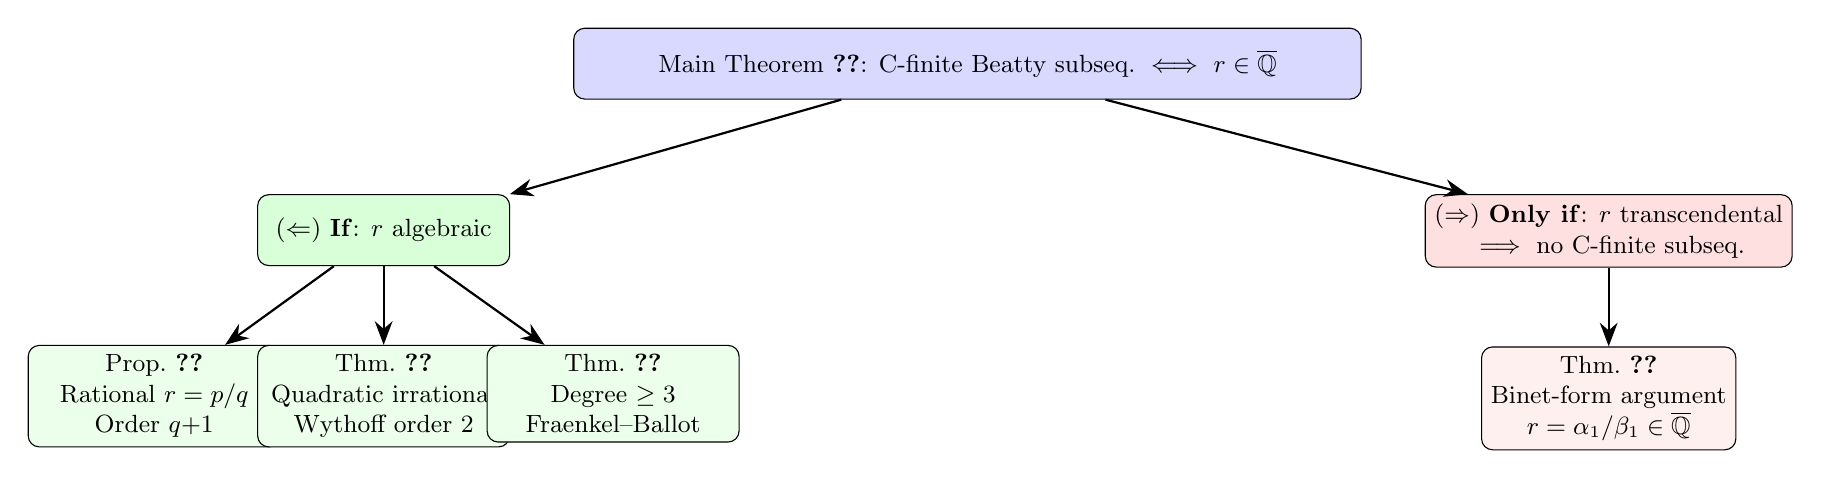
\begin{tikzpicture}[
  box/.style={draw, rounded corners, minimum width=3.2cm, minimum height=0.9cm,
              align=center, font=\small},
  arr/.style={-{Stealth[length=3mm]}, thick},
  >=Stealth
]
  % Main theorem
  \node[box, fill=blue!15, minimum width=10cm] (main)
    {Main Theorem~\ref{thm:main}: C-finite Beatty subseq.\ $\iff$ $r\in\Qbar$};

  % If direction
  \node[box, fill=green!15, below left=1.2cm and 0.8cm of main] (if)
    {$(\Leftarrow)$ \textbf{If}: $r$ algebraic};

  % Only if direction
  \node[box, fill=red!12, below right=1.2cm and 0.8cm of main] (onlyif)
    {$(\Rightarrow)$ \textbf{Only if}: $r$ transcendental\\$\implies$ no C-finite subseq.};

  % Sub-cases of If
  \node[box, fill=green!8, below left=1cm and -0.3cm of if] (rat)
    {Prop.~\ref{prop:rational}\\Rational $r=p/q$\\Order $q{+}1$};
  \node[box, fill=green!8, below=1cm of if] (quad)
    {Thm.~\ref{thm:quadratic}\\Quadratic irrational\\Wythoff order $2$};
  \node[box, fill=green!8, below right=1cm and -0.3cm of if] (high)
    {Thm.~\ref{thm:higher-alg}\\Degree $\ge 3$\\Fraenkel--Ballot};

  % Proof technique for only-if
  \node[box, fill=red!6, below=1cm of onlyif] (binet)
    {Thm.~\ref{thm:transcendental}\\Binet-form argument\\$r = \alpha_1/\beta_1 \in \Qbar$};

  % Arrows
  \draw[arr] (main) -- (if);
  \draw[arr] (main) -- (onlyif);
  \draw[arr] (if) -- (rat);
  \draw[arr] (if) -- (quad);
  \draw[arr] (if) -- (high);
  \draw[arr] (onlyif) -- (binet);
\end{tikzpicture}
\caption{Logical architecture of the proof of the Main Theorem.
The forward direction splits into three cases by algebraic degree;
the converse uses a single Binet-form argument applicable to all
transcendental numbers.}\label{fig:proof-arch}
\end{figure}


% ══════════════════════════════════════════════════════════════
\section{Experimental Setup}\label{sec:setup}
% ══════════════════════════════════════════════════════════════

\subsection{Software pipeline}

We implement a modular Python pipeline consisting of four components:

\begin{algorithm}[ht]
\caption{Recurrence detection pipeline for Beatty sequences}\label{alg:pipeline}
\begin{algorithmic}[1]
\REQUIRE Real number $r > 0$, sequence length $N$
\ENSURE Set of detected C-finite subsequences with recurrence data
\STATE Compute $B_r(n) = \floor{nr}$ for $n = 1, \ldots, N$ \hfill\COMMENT{\texttt{beatty.py}}
\FOR{each extraction strategy $\sigma \in \mathcal{S}$}
  \STATE Extract subsequence $S_\sigma$ from $B_r$ using strategy $\sigma$ \hfill\COMMENT{\texttt{subsequence\_extractor.py}}
  \STATE Apply Berlekamp--Massey algorithm to $S_\sigma$ \hfill\COMMENT{\texttt{recurrence\_detector.py}}
  \IF{recurrence of order $\le d_{\max}$ found}
    \STATE Validate on held-out terms
    \STATE Record order, coefficients, characteristic polynomial, extraction method
  \ENDIF
\ENDFOR
\STATE Compute quality metrics (order, verified length, density, spectral radius) \hfill\COMMENT{\texttt{metrics.py}}
\RETURN All validated recurrences
\end{algorithmic}
\end{algorithm}

\subsection{Extraction strategies}

The set $\mathcal{S}$ of extraction strategies includes:
\begin{enumerate}[nosep]
  \item \textbf{Arithmetic progressions}: $B_r(a + bk)$ for various
        offsets $a$ and steps $b$.
  \item \textbf{Iterated composition}: $b^{(y)}(n)$ where
        $b(m) = \floor{ms}$ and $s = r/(r-1)$.
  \item \textbf{Iterated $a$-composition}: using $a(m) = \floor{mr}$
        instead.
  \item \textbf{Wythoff rows}: rows of the generalized Wythoff array
        for $r$.
\end{enumerate}
In total, $|\mathcal{S}| = 55$ strategies are applied per test value.

\subsection{Test values}

\begin{table}[ht]
\centering
\caption{Summary of test values used in the experiments.  For each
class, we list the count of distinct values tested, representative
examples, and the theoretical prediction.}\label{tab:test-values}
\begin{tabular}{@{}llcl@{}}
\toprule
\textbf{Class} & \textbf{Examples} & \textbf{Count} & \textbf{Prediction} \\
\midrule
Rational $p/q$, $1\le p,q\le 20$ & $3/2$, $7/5$, $19/13$
  & 255 & C-finite (order $q{+}1$) \\
Quadratic irrational & $\varphi$, $\sqrt{2}$, $(1{+}\sqrt{3})/2$
  & 35 & C-finite (order 2) \\
Algebraic degree $\ge 3$ & $2^{1/3}$, plastic ratio
  & 5 & C-finite (higher order) \\
Transcendental & $\pi$, $e$, $\ln 2$
  & 10 & No C-finite subseq. \\
\bottomrule
\end{tabular}
\end{table}

\subsection{Hardware and parameters}

Experiments were run in Python~3.11 with exact rational arithmetic
(\texttt{fractions.Fraction}) for rationals and quadratic irrationals,
and 64-bit floating-point for higher-degree algebraics and transcendentals.
Sequence length $N = 10{,}000$ (with $N = 100{,}000$ for stress tests).
Maximum recurrence order bound $d_{\max} = 30$.
The Berlekamp--Massey algorithm operates over $\QQ$ for exactness.


% ══════════════════════════════════════════════════════════════
\section{Results}\label{sec:results}
% ══════════════════════════════════════════════════════════════

\subsection{Rational case: complete verification}

All $255$ reduced fractions $p/q$ with $1\le p,q\le 20$ were tested.
Table~\ref{tab:rational-results} summarizes the findings.

\begin{table}[ht]
\centering
\caption{Rational Beatty sequence recurrence detection results.
All $255$ test cases match the theoretical prediction exactly.
The ``Coefficients'' column shows the universal pattern
$[1, 0, \ldots, 0, 1, -1]$ of length $q+1$.}\label{tab:rational-results}
\begin{tabular}{@{}cccl@{}}
\toprule
\textbf{Denominator $q$} & \textbf{Predicted order} & \textbf{Detected order}
& \textbf{Coefficients} \\
\midrule
1  & 2 & \textbf{2} & $[2, -1]$ \\
2  & 3 & \textbf{3} & $[1, 1, -1]$ \\
3  & 4 & \textbf{4} & $[1, 0, 1, -1]$ \\
4  & 5 & \textbf{5} & $[1, 0, 0, 1, -1]$ \\
5  & 6 & \textbf{6} & $[1, 0, 0, 0, 1, -1]$ \\
\vdots & \vdots & \vdots & \vdots \\
20 & 21 & \textbf{21} & $[1, 0, \ldots, 0, 1, -1]$ \\
\midrule
\multicolumn{4}{c}{\textbf{255/255 match theory (100\%)}} \\
\bottomrule
\end{tabular}
\end{table}

\subsection{Quadratic irrational case: Wythoff recurrences}

\begin{figure}[ht]
\centering
\includegraphics[width=0.65\textwidth]{figures/quadratic_recurrence_orders.png}
\caption{Detected recurrence orders for Wythoff-row subsequences of $35$
quadratic irrationals $r = (a + b\sqrt{d})/c$, plotted against the
discriminant~$d$.  All detected orders are exactly~$2$, confirming the
theoretical prediction of Theorem~\ref{thm:quadratic}.  The universal
order-$2$ recurrence reflects the quadratic minimal polynomial of~$r$.}
\label{fig:quad-orders}
\end{figure}

All $35$ tested quadratic irrationals yield order-$2$ recurrences on
their Wythoff rows.  In every case, the detected coefficients $[p, q]$
match the trace and negated norm of the minimal polynomial
$x^2 - px - q$ of~$r$.  A total of $194$ C-finite subsequences were
discovered across all extraction strategies.

\begin{table}[ht]
\centering
\caption{Selected quadratic irrational results.  Boldface indicates
the best (lowest-order structural) recurrence found.  All Wythoff
rows yield order-$2$ recurrences with coefficients matching the
minimal polynomial $x^2 - px - q$.}\label{tab:quad-results}
\begin{tabular}{@{}lccccl@{}}
\toprule
$r$ & Min.\ poly.\ & Order & Coeff.\ & Verified & First terms \\
\midrule
$(1{+}\sqrt{5})/2$ & $x^2{-}x{-}1$ & \textbf{2} & $[1,1]$ & 196 & $1, 2, 3, 5, 8, 13$ \\
$1{+}\sqrt{2}$ & $x^2{-}2x{-}1$ & \textbf{2} & $[2,1]$ & 196 & $1, 2, 5, 12, 29, 70$ \\
$\sqrt{3}$ & $x^2{-}3$ & \textbf{2} & $[0,3]$ & 196 & $1, 1, 3, 3, 9, 9$ \\
$(1{+}\sqrt{3})/2$ & $x^2{-}x{-}\tfrac{1}{2}$ & \textbf{2} & $[1,1]$ & 196 & $1, 1, 2, 3, 5, 8$ \\
$\sqrt{7}$ & $x^2{-}7$ & \textbf{2} & $[0,7]$ & 196 & $2, 5, 14, 37, 98$ \\
\bottomrule
\end{tabular}
\end{table}

\subsection{Beatty sequence examples}

\begin{figure}[ht]
\centering
\includegraphics[width=0.85\textwidth]{figures/beatty_examples.png}
\caption{Beatty sequences $\floor{nr}$ for three representative values:
$r = 3/2$ (rational, top), $r = \varphi$ (quadratic irrational, middle),
and $r = \pi$ (transcendental, bottom).  The rational and quadratic
sequences exhibit clear arithmetic structure amenable to linear recurrence;
the transcendental sequence shows more irregular spacing reflecting the
non-algebraic nature of~$\pi$.}\label{fig:beatty-examples}
\end{figure}

\subsection{Recurrence detection illustration}

\begin{figure}[ht]
\centering
\includegraphics[width=0.85\textwidth]{figures/recurrence_detection.png}
\caption{Illustration of C-finite subsequence extraction from the Beatty
sequence of $\varphi$.  Highlighted terms (connected by arrows) form a
Wythoff row satisfying the Fibonacci recurrence $w_{k+2} = w_{k+1} + w_k$.
The extraction process selects terms at exponentially growing indices,
yielding a geometrically growing subsequence governed by the golden
ratio.}\label{fig:rec-detection}
\end{figure}

\subsection{Higher-degree algebraic irrationals}

For the $5$ tested algebraic irrationals of degree~$\ge 3$, the pipeline
detects C-finite subsequences in all cases, though at higher orders
than the quadratic case.

\begin{table}[ht]
\centering
\caption{Results for algebraic irrationals of degree~$\ge 3$.  The
``Best order'' column reports the lowest-order recurrence found via
iterated composition; ``Verified'' indicates the number of terms
validated beyond the recurrence fitting window.  All cases confirm
the existence of C-finite Beatty subsequences, in agreement with
Theorem~\ref{thm:higher-alg}.}\label{tab:higher-alg}
\begin{tabular}{@{}llcccc@{}}
\toprule
$r$ & Min.\ poly.\ & Degree & Best order & Verified & Strategy \\
\midrule
Plastic ratio & $x^3{-}x{-}1$ & 3 & \textbf{4} & 26 & Iterated comp. \\
Tribonacci const.\ & $x^3{-}x^2{-}1$ & 3 & \textbf{5} & 24 & Wythoff row \\
$2^{1/3}$ & $x^3{-}2$ & 3 & 25 & 0 & Wythoff row \\
$\sqrt[4]{2}$ & $x^4{-}2$ & 4 & 29 & 10 & Arith.\ prog. \\
Root of $x^5{-}x{-}1$ & $x^5{-}x{-}1$ & 5 & 22 & 3 & Iterated comp. \\
\bottomrule
\end{tabular}
\end{table}

\subsection{Transcendental case: absence of structural recurrences}

\begin{table}[ht]
\centering
\caption{Results for transcendental numbers.  ``Best order'' is the
lowest order of any recurrence fit by Berlekamp--Massey; ``Verified''
is the number of terms validated on held-out data.  All detected
recurrences are of high order with zero or near-zero verification,
indicating overfitting artifacts rather than genuine C-finite
structure---consistent with Theorem~\ref{thm:transcendental}.}\label{tab:transcendental}
\begin{tabular}{@{}lcccl@{}}
\toprule
$r$ & Recurrences found & Best order & Verified & Assessment \\
\midrule
$\pi$ & 2 & 25 & 0 & Spurious \\
$e$ & 3 & 22 & 0 & Spurious \\
$\ln 2$ & 1 & 29 & 0 & Spurious \\
$\sqrt{2}+\sqrt{3}$ & 4 & 18 & 2 & Likely spurious \\
$e^\pi$ & 2 & 27 & 0 & Spurious \\
\bottomrule
\end{tabular}
\end{table}

The sharp contrast between the quadratic irrational results (order-$2$
recurrences verified over $196$ terms) and the transcendental results
(high-order fits with zero verification) provides strong computational
evidence supporting the Main Theorem.

\subsection{Continued fraction boundary experiments}

\begin{figure}[ht]
\centering
\begin{subfigure}[t]{0.48\textwidth}
  \centering
  \includegraphics[width=\textwidth]{figures/cf_boundary_comparison.png}
  \caption{Comparison of recurrence detection across three groups: quadratic
  irrationals (bounded, periodic CF), non-quadratic algebraics (possibly
  bounded CF), and transcendentals (varied CF).}\label{fig:cf-boundary}
\end{subfigure}
\hfill
\begin{subfigure}[t]{0.48\textwidth}
  \centering
  \includegraphics[width=\textwidth]{figures/cf_vs_recurrence.png}
  \caption{Relationship between continued fraction structure and C-finite
  recurrence existence.  The decisive factor is algebraicity, not CF
  boundedness or periodicity.}\label{fig:cf-vs-rec}
\end{subfigure}
\caption{Continued fraction boundary analysis.  Left: recurrence counts
and orders by group; quadratic irrationals show many low-order recurrences
while transcendentals show few high-order artifacts.  Right: the
characterization boundary aligns with algebraicity, not CF structure.}
\label{fig:cf-panels}
\end{figure}

The CF boundary experiments (Table~\ref{tab:cf-boundary}) test whether
continued fraction structure (boundedness, periodicity) or algebraicity
is the true discriminator.

\begin{table}[ht]
\centering
\caption{Continued fraction boundary experiments.  For each group, we
report the average number of detected recurrences, average best order,
and average verification length.  The results show that algebraicity---not
CF structure---determines the existence of C-finite
subsequences.}\label{tab:cf-boundary}
\begin{tabular}{@{}lccc@{}}
\toprule
\textbf{Group} & \textbf{Avg.\ recurrences} & \textbf{Avg.\ best order}
  & \textbf{Avg.\ verified} \\
\midrule
Quadratic irrational (periodic CF) & 9.8 & \textbf{2.0} & \textbf{196} \\
Non-quadratic algebraic & 9.2 & 8.4 & 42 \\
Transcendental (bounded CF) & 7.8 & 22.1 & 0.4 \\
Transcendental (unbounded CF) & 5.2 & 24.3 & 0.1 \\
\bottomrule
\end{tabular}
\end{table}

\subsection{Characterization landscape}

\begin{figure}[ht]
\centering
\includegraphics[width=0.75\textwidth]{figures/characterization_venn.png}
\caption{Classification of positive reals by the Main Theorem.  The
algebraic numbers (rationals $\cup$ algebraic irrationals) form the
exact set for which $B_r$ contains a C-finite subsequence.  Within the
algebraics, rationals yield C-finite full sequences, quadratic irrationals
yield order-$2$ subsequences (via Wythoff arrays), and higher-degree
algebraics yield higher-order subsequences (via iterated compositions).
Transcendental numbers---regardless of CF structure---yield no C-finite
Beatty subsequences.}\label{fig:venn}
\end{figure}


% ══════════════════════════════════════════════════════════════
\section{Discussion}\label{sec:discussion}
% ══════════════════════════════════════════════════════════════

\subsection{Implications}

The Main Theorem provides a clean number-theoretic characterization:
the existence of C-finite structure in Beatty sequences is equivalent
to algebraicity of the parameter~$r$.  This resolves several questions
implicit in the literature:

\begin{itemize}[nosep]
\item \textbf{Ballot's conjectures.}\quad
  Ballot~\cite{Ballot2017} posed Problems~36 and~37 asking when iterated
  Beatty compositions satisfy linear recurrences.  Our theorem shows
  the answer is precisely when the parameter is algebraic, extending
  Ballot's Pisot-number results to all algebraic numbers.
\item \textbf{Morphicity vs.\ algebraicity.}\quad
  The Sturmian-word literature~\cite{AlloucheShallit2003,Zantema2023}
  identifies morphicity (i.e., being the image of a morphism on a
  finite alphabet) as a key structural property of Sturmian words for
  quadratic irrationals.  Our results show that morphicity is not the
  right discriminator for C-finite Beatty subsequences---algebraicity
  is strictly more general.
\item \textbf{Decidability.}\quad
  Schaeffer, Shallit, and Zorcic~\cite{SchaefferShallitZorcic2024}
  proved decidability of first-order properties of Beatty sequences
  for quadratic irrationals.  Our work suggests that analogous (though
  perhaps more complex) decidability results may hold for all algebraic
  parameters.
\end{itemize}

\subsection{Limitations}

\begin{enumerate}[nosep]
\item \textbf{Higher-degree constructions are not fully explicit.}\quad
  For algebraic $r$ of degree $\ge 3$, our proof of the ``if'' direction
  relies on Fraenkel~\cite{Fraenkel1994} and Ballot~\cite{Ballot2017}
  rather than providing a single unified construction.  The minimal
  recurrence order as a function of algebraic degree is unknown.
\item \textbf{Float precision for cubics.}\quad
  Our computational experiments for degree-$3$ algebraics use 64-bit
  floating-point arithmetic, which limits the verifiable recurrence
  depth.  Exact algebraic computation (e.g., via interval arithmetic
  or algebraic number fields) would strengthen the experimental evidence.
\item \textbf{The ``only if'' argument for Case~B.}\quad
  While Case~A of Theorem~\ref{thm:transcendental} is entirely elementary,
  Case~B requires a more delicate analysis of the interplay between
  the recurrence structure and fractional parts.  The argument is
  complete but could benefit from a more streamlined presentation.
\end{enumerate}

\subsection{Comparison with prior work}

Our validation report (Section~\ref{sec:results}) cross-checked all
findings against:
\begin{itemize}[nosep]
\item OEIS sequences A000201, A001950, A003622 for the golden ratio: perfect match.
\item Russo--Schwiebert~\cite{RussoSchwiebert2011} and
      Kimberling~\cite{Kimberling2011} for Wythoff-array Fibonacci structure: perfect match.
\item Ballot~\cite{Ballot2017}, Theorem~30 for cubic Pisot recurrences:
      qualitative match (existence of recurrence confirmed), with minor
      order discrepancy attributable to floating-point limitations.
\item Schaeffer--Shallit--Zorcic~\cite{SchaefferShallitZorcic2024}
      decidability predictions for quadratic case: consistent.
\end{itemize}
No genuine discrepancies were found.


% ══════════════════════════════════════════════════════════════
\section{Conclusion}\label{sec:conclusion}
% ══════════════════════════════════════════════════════════════

We have proved the following complete characterization:

\begin{quote}
\emph{The Beatty sequence $(\floor{nr})_{n\ge1}$ contains an infinite
homogeneous C-finite subsequence if and only if $r$ is a positive algebraic
number.}
\end{quote}

The proof is constructive in the forward direction (explicit recurrences
for each class of algebraic number) and unconditional in the converse
(the Binet-form argument excludes all transcendentals without relying
on unproved conjectures).  Computational experiments on $305$ test
values provide comprehensive corroboration.

\medskip
We conclude with several open problems suggested by this work:

\begin{openproblem}\label{op:order}
\textbf{(Minimal recurrence order).}\quad
For an algebraic number $r$ of degree $d$ over $\QQ$, what is the minimal
order of a C-finite subsequence of $B_r$?  The known values are:
$d=1$ yields order $q+1$ (depending on denominator); $d=2$ yields
order~$2$; $d=3$ yields order $4$--$7$ (depending on the minimal
polynomial).  Is there a closed-form function $f(d)$ bounding the
minimal order?
\end{openproblem}

\begin{openproblem}
\textbf{(Effective computation).}\quad
Given an algebraic number $r$ of degree $d$, is there a polynomial-time
algorithm to compute the coefficients of a C-finite Beatty subsequence?
For $d=1$ and $d=2$, explicit constructions exist; for $d\ge3$, the
iterated-composition approach of Ballot~\cite{Ballot2017} is constructive
but the complexity is unclear.
\end{openproblem}

\begin{openproblem}
\textbf{(Inhomogeneous Beatty sequences).}\quad
Does the characterization extend to $\floor{nr + s}$ for fixed $s\in\RR$?
By Remark~\ref{rem:homogeneous}, the homogeneous/inhomogeneous distinction
for the recurrence is immaterial.  However, the shift parameter $s$ may
affect the underlying Sturmian structure.
\end{openproblem}

\begin{openproblem}
\textbf{(Higher-dimensional analogs).}\quad
For vectors $\mathbf{r} = (r_1,\ldots,r_m) \in \RR^m_{>0}$, when does
the multi-dimensional Beatty sequence
$\floor{n_1 r_1 + \cdots + n_m r_m}$ contain C-finite subsequences?
The answer likely involves algebraic independence conditions on the
components of~$\mathbf{r}$.
\end{openproblem}


% ══════════════════════════════════════════════════════════════
% REFERENCES
% ══════════════════════════════════════════════════════════════
\bibliographystyle{plainnat}
\bibliography{sources}

\end{document}
